%Lezione 01
\chapter{Introduzione}
L'automazione è una disciplina estremamente ampia, si intende in questo corso con
\textit{automazione} la progettazione, la realizzazione e la gestione di sistemi in grado di
eseguire dei compiti in maniera autonoma, senza l'intervento dell'uomo.

Nel corso verranno effettuate le analisi di sistemi dinamici, con un focus finale sulle analisi di
sistemi di controllo che verranno approfondite al corso di ``controlli''.

L'uomo ha sempre cercato di automatizzare i processi o i compiti che doveva eseguire, per ridurre
la fatica e l'usura per le attività manuali.

Un esempio è il \textbf{regolatore di Watt}, una macchina in grado di regolare il grado di
ammissione di una valvola di alimentazione per una macchina a vapore, al fine di mantenere costante
la velocità di rotazione della macchina.

Inizialmente l'operazione era compiuta da un operatore che regolava la temperatura della caldaia
fornendo più o meno combustibile.

Quest'oggetto racchiude l'essenza dei controlli automatici:
\begin{itemize}
 \item Elemento di trasduzione e misura, fondamentale per ottenere informazioni sulla grandezza da
controllare, in questo caso la velocità di rotazione delle macchine da controllare. L'uscita dello
strumento di misura può essere di diversa natura rispetto alla grandezza misurata ma comunque
proporzionale ad esso.
 \item Elemento di controllo (controllore), in questo caso il sistema di leve e pesi che varia la
posizione del cursore in funzione dell'input e delle sue caratteristiche come i pesi e le lunghezze
delle leve.
\item Attuatore, ossia uno strumento in grado di attuare la decisione del controllore sul sistema,
nel caso precedente la valvola.
\end{itemize}

Nel contesto più generale dei sistemi dinamici si riuscirà a modellare ed analizzare i sistemi
dinamici in generale e comprendere le proprietà fondamentali e strutturali dei sistemi studiati.

\section{Sistemi dinamici}
Un sistema è qualunque oggetto o processo materiale o immateriale, ben delimitato nel suo
funzionamento.
Potrebbe essere un sistema meccanico o termico, o ad esempio un sistema immateriale come
l'andamento del PIL in Italia.

Gli oggetti di interesse in particolare sono quelli \textit{dinamici}
che hanno ossia la possibilità di variare nel tempo alcune grandezze che li caratterizzano.

L'unica variabile indipendente considerata nell'intero corso sarà il tempo, anche i sistemi
astratti saranno comunque sistemi ``esistenti''.

Dato un certo sistema si dovrà astrarre dal sistema un modello che lo rappresenta,
operazione denominata modellistica, il modello prende il nome di \textbf{oggetto astratto
orientato}.

Con ``identificazione dei sistemi dinamici'' si intende la scienza che permette la costruzione di
modelli matematici anche quando i sistemi in esame e le loro proprietà fisiche non sono note.

Costruito il modello è poi possibile analizzare le caratteristiche dell'oggetto, attraverso la
quale si possono conoscere le caratteristiche comportamentali del modello.

Le previsioni meteorologiche sono un classico esempio di analisi in un sistema dinamico, va
modellato il pianeta in funzione del fenomeno da studiare, vanno quindi determinate le variabili
inerenti il fenomeno. Esiste un modello matematico del pianeta che permette di prevedere le
grandezze future del sistema dato lo stato attuale dello stesso.

Se si esegue ad esempio l'analisi del modello termico di una stanza si ottiene un valore di
temperatura diverso da quello desiderato e corrispondente al comportamento naturale del sistema.
Se si desidera un valore di temperatura differente, va costruito un sistema di condizionamento e
controllo che con un attuatore modifichi l'evoluzione del sistema.

\section{Oggetto astratto orientato}
È un'astrazione di un oggetto reale, dal quale si ricavano un insieme di equazioni e variabili che
ne descrivano le grandezze di interesse.
È un modello \textit{parziale} della realtà, sia perché analizza solo uno o una parte di fenomeno,
sia perché, anche nella grandezza di interesse, non sarà mai identico alla realtà a causa delle
varie approssimazioni.

L'accuratezza di un modello solitamente aumenta all'aumentare della complessità del modello, va
determinato il grado di complessità in funzione dell'accuratezza richiesta al risultato.

Con il termine \textit{orientato} si intende sottolineare che il modello matematico deve essere un
modello \textbf{causale}, ossia che rispetti il principio di causa-effetto, l'effetto
\textit{segue} nel tempo la causa, altrimenti sarebbe un sistema che prevede il futuro. In alcune
discipline si studiano anche sistemi non causali, come ad esempio nella trasmissione digitale
terrestre possono essere utilizzati dei filtri anti-causali, trasmettendo ad esempio il segnale con
una latenza di tre secondi, è possibile sfruttare questi secondi di ``buffer'' per ricostruire in
maniera più accurata il segnale.

Il concetto di ``orientato'' fa nascere un'idea discriminante nell'ambito delle variabili presenti
nel modello, dividendole in due grandi \textit{famiglie}, ossia
\textbf{ingresso} o \textbf{uscita}.

Si identificano con \textit{u} le variabili di ingresso e con \textit{y} quelle di uscita.
\begin{figure}[h]
 \centering
 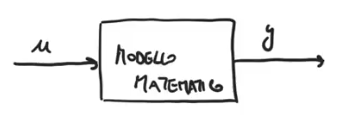
\includegraphics[width=\picwid]{modello_matematico.png}
 % modello_matematico.png: 341x119 px, 96dpi, 9.02x3.15 cm, bb=0 0 256 89
 \label{Fig.:modello_matematico}
\end{figure}

\subsection{Esempio di una rete RLC}
Si considera il seguente sistema
 \begin{figure}[h]
 \centering
 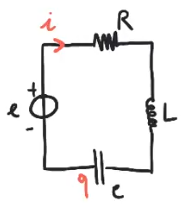
\includegraphics[width=\picwid]{rete_RLC_esempio1.png}
 % rete_RLC_esempio1.png: 190x214 px, 96dpi, 5.03x5.66 cm, bb=0 0 142 160
 \label{Fig.:circuito_RLC}
\end{figure}
Si scrive l'equazione alla maglia
\begin{equation}
 e = R \dot{q} + L\ddot{q} + \frac{q}{C}
 \label{eq:equazione_RLC}
\end{equation}
con $q$ la carica elettrica e la notazione $\dot{q}$ per indicare la derivata prima nel tempo,
$\ddot{q}$ la seconda e così via.

Sono presenti due variabili nell'equazione, una di ingresso e una di uscita, un oggetto astratto
orientato che soddisfa la proprietà di casualità (generatore $\rightarrow$ carica)

\newpage
\subsection{Esempio di una sospensione di un'autovettura}
Il seguente sistema può essere schematizzato come una massa collegata ad una molla in
\textit{parallelo} ad uno smorzatore idraulico (pistone).
\begin{figure}[h]
 \centering 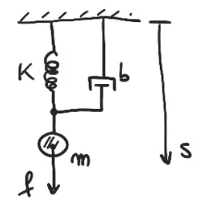
\includegraphics[width=\picwid]{massa_molla_smorzatore.png}
 % massa_molla_smorzatore.png: 133x166 px, 96dpi, 3.52x4.39 cm, bb=0 0 100 124
 \label{Fig.:massa_molla_smorzatore}
\end{figure}

È possibile costruire il modello matematico del sistema applicando il secondo principio della
dinamica a ciascuna massa in gioco e per ciascun grado di libertà della stessa.
Si suppone che la massa possa muoversi solo lungo la direzione verticale e si indica con $s$ la sua
posizione, di conseguenza $\dot{s}$ sarà la velocità e $\ddot{s}$ l'accelerazione.
\begin{equation}
 m\ddot{s} = f - ks - b\dot{s}
 \label{eq:equazione_massa_molla_smorzatore}
\end{equation}
dove $k$ è la rigidezza della molla e $b$ la viscosità dello smorzatore riferita alla velocità.

I due sistemi sono eterogenei tra loro, ma possono essere facilmente messi in relazione nel
seguente modo:
$$
\begin{aligned}
m &\leftrightarrow L\\
b &\leftrightarrow R\\
k &\leftrightarrow \frac{1}{C}\\
s &\leftrightarrow q\\
f &\leftrightarrow e
\end{aligned}
$$

Se si sostituissero i termini della
\ref{eq:equazione_massa_molla_smorzatore}
 nella \ref{eq:equazione_RLC} si otterrebbe ancora la stessa equazione, ciò mostra che due sistemi
completamente differenti tra loro possono dare origine ad un modello astratto identico.
Dal punto di vista di oggetto astratto, sono dunque lo stesso sistema, ossia il comportamento di
uno può essere associato allo stesso comportamento dell'altro.

\newpage
\section{Variabili di ingresso e uscita}
\subsection{Massa su un piano}
Si vuole trovare un metodo per determinare le variabili di ingresso e uscita di un sistema.

Sia dato il seguente sistema composto da una massa $m$ posta su un piano e sottoposta ad una forza
$f$ di equazione
\begin{equation}
 m\ddot{s} = f
\end{equation}
è immediato constatare che la forza sia l'ingresso e lo spostamento l'uscita, non può esserci
spostamento senza forza.
\subsection{Bilancio familiare}
Si consideri un ``sistema'' formato da un nucleo familiare, la prima grandezza è \textit{l'introito
mensile} mentre un'altra variabile è il \textit{tenore di vita}, non è in questo caso facile
determinare l'equazione che lega queste due variabili.

Sarà intuitivo constatare che \textit{l'introito} sarà la variabile di ingresso e il \textit{tenore
di vita} la variabile di uscita.

\subsection{Capacitore}
Si consideri un semplice capacitore attraversato da una corrente $i$ e una tensione ai suoi capi
pari a $v$, non è in questo caso immediato trovare la variabile di ingresso e quella di uscita.
$$
q = C\cdot v
$$
Ragionando sul fenomeno fisico si vede che è la carica $q$ (e dunque la corrente) a determinare la
tensione ai capi del condensatore e non il viceversa, questo ragionamento richiede però la
conoscenza del fenomeno fisico in esame e non può essere generalizzato a tutti i sistemi.

\subsection{Regola generale}
Un caso comune è l'analisi di sistemi a partire già dal modello matematico, senza conoscere in
alcun modo il processo fisico.
Osservando unicamente le equazioni è possibile determinare quali siano le variabili di ingresso e
uscita, questo è possibile grazie ad uno strumento che discende direttamente dal principio di
causalità:\newline
\emph{saranno variabili di ingresso quelle che compaiono differenziate un numero
inferiore di volte all'interno dell'equazione del sistema.}
\newline
Tutte le altre \textit{possono} essere variabili di uscita.
Non è detto che ai fini dello studio interessino tutte le variabili non di ingresso.
